\documentclass[conference]{IEEEtran}

% Packages
    \usepackage{times}

    % numbers option provides compact numerical references in the text. 
    \usepackage[numbers]{natbib}
    \usepackage{multicol}
    \usepackage[bookmarks=true]{hyperref}
    \usepackage{multirow}
    \usepackage{tikz} % graphical models
    \usetikzlibrary{chains,fit,shapes}
    \usetikzlibrary{bayesnet}

    \usepackage{amsmath,amsfonts,amsthm,amssymb,amsopn,bm} %%% load AMS-Latex Package
    \usepackage{graphics,graphicx,subfigure,color} %figures and color   
    \usepackage{mathrsfs}

% Commands
    \newcommand{\figref}[1]{Fig.~\ref{#1}}
    \newcommand{\secref}[1]{Sec.~\ref{#1}}	
	\renewcommand{\eqref}[1]{Eq.~(\ref{#1})}
	\newcommand{\tabref}[1]{Tab.~\ref{#1}}
	\newcommand{\algref}[1]{Algorithm~\ref{#1}}

    \newcommand{\prob}[1]{\text{p}(#1)} % probability
    \newcommand{\set}[1]{\mathbf{#1}} % Capital set bold letter
    \newcommand{\italic}[1]{\textit{#1}} % italic
    \newcommand{\boldface}[1]{\textbf{#1}} % bold
    \newcommand{\cursive}[1]{\mathcal{#1}}
    \newcommand{\script}[1]{\mathscr{#1}}
    \DeclareMathOperator*{\argmin}{argmin}
    \DeclareMathOperator*{\argmax}{argmax}
    \newcommand{\entropy}[1]{\text{H}\left[\;#1 \; \right]} % entropy
    \newcommand{\expectedValue}[2]{\hollow{E}_{#2}#1} % expected value
    \newcommand{\hollow}[1]{\mathbb{#1}} % hollow letter

%\pdfinfo{
%   /Author (Homer Simpson)
%   /Title  (Robots: Our new overlords)
%   /CreationDate (D:20101201120000)
%   /Subject (Robots)
%   /Keywords (Robots;Overlords)
%}

\begin{document}

% Cover Page
    % paper title
    \title{Towards Interactive Object Recognition}

    % You will get a Paper-ID when submitting a pdf file to the conference system
    \author{Author Names Omitted for Anonymous Review. Paper-ID [add your ID here]}

    %\author{\authorblockN{Karol Hausman}
    %\authorblockA{Robotic Embedded Systems Group\\
    %University of Southern California\\
    %Los Angeles, CA 30332--0250\\
    %Email: mshell@ece.gatech.edu}
    %\and
    %\authorblockN{Homer Simpson}
    %\authorblockA{Twentieth Century Fox\\
    %Springfield, USA\\
    %Email: homer@thesimpsons.com}
    %\and
    %\authorblockN{James Kirk\\ and Montgomery Scott}
    %\authorblockA{Starfleet Academy\\
    %San Francisco, California 96678-2391\\
    %Telephone: (800) 555--1212\\
    %Fax: (888) 555--1212}}


    % avoiding spaces at the end of the author lines is not a problem with
    % conference papers because we don't use \thanks or \IEEEmembership


    % for over three affiliations, or if they all won't fit within the width
    % of the page, use this alternative format:
    \author{\authorblockN{Karol Hausman,
    Chet Corcos, J\"{o}rg M\"{u}ller,
    Fei Sha and 
    Gaurav S. Sukhatme}\\
    \authorblockA{University of Southern California\\
    Department of Computer Science,\\
    {\texttt{\{hausman, corcos, joerg.mueller, feisha, gaurav\}@usc.edu}}}}

    \maketitle

\begin{abstract}
%    This paper starts with a probabilitic Bayesian Network approach to predict objects and poses for any variety of extracted features. This basic object recognition model is extended to incorporate actions over time. An optimal solution is derived for determining the best action for expected object recognition in future predictions.   
% let's leave the abstract out for now. This is the most important part. Let's write it at the end.
\end{abstract}

\IEEEpeerreviewmaketitle

\section{Introduction}

    %* show the problem
    %* introduce the idea
    %* contributions?

    % introduce the problem
    Many state-of-the-art object recognition systems have been developed using a variety of feature extraction techniques. Despite the fact that some of them have been very successful, we still cannot say that the problem of object recognition has been solved. We claim that the reason for that is already included in the problem formulation. Given static images there are cases where it is impossible to recognize the object as it may appear ambiguous with respect to another object(see~\figref{fig:pr2}). One of the reasons for that is that distinctive features may be hidden due to the pose of the object.  In this paper we present an approach to help tackle this problem.
    
    % introduce the idea
    In this work we take advantage of robot's manipulation capabilities and apply them in the domain of object recognition. In our approach we tackle interactive object recognition problem where we look for the action that will minimize the expected entropy over objects distribution. Therefore we want to be optimal in the number of actions that will lead us to successful object recognition.

	% contributions
	The key contributions of our approach are that (a) to the best of our knowledge, we are first to introduce the idea of a robot interacting with the scene in order to improve object recognition, (b) our approach is probabilistic and takes into account a probabilistic object recognition model that is agnostic to the feature type, (c) we present an action selection model that reasons about the most informative action which leads to optimality in the number of actions to recognize the object.
	
	
    
    \setlength{\tabcolsep}{0.1em}
    \begin{figure}[ht]
    \begin{tabular}{cccc}
    \multicolumn{2}{c}{\multirow{-5}{*}{\includegraphics[width=0.46\columnwidth]{pics/pr2_init.jpg}}} & \includegraphics[width=0.23\columnwidth]{pics/first_back.jpg} 
    &\includegraphics[width=0.23\columnwidth]{pics/first_cover1.jpg} \\
    \multicolumn{2}{c}{} & \includegraphics[width=0.23\columnwidth]{pics/first_back.jpg} 
    &\includegraphics[width=0.23\columnwidth]{pics/first_cover2.jpg} \\
    \multicolumn{2}{c}{\includegraphics[width=0.45\columnwidth]{pics/pr2_grasp.jpg}}
    & \multicolumn{2}{c}{\includegraphics[width=0.45\columnwidth]{pics/pr2_rotate.jpg}}
    \end{tabular}
    \caption{Top-left: The service robot PR2 trying to recognize a book based on the back. Database of objects consists of book 1 (top-right, NE and NW) and book 2, (top-right, SE and SW) that look the same from the back. PR2 has to take the optimal action in order to recognize which book it is. In this case it means it flips it over(bottom-left, bottom-right).}
    \label{fig:pr2}
    \end{figure}

    %contributions
    %* novel probabilistic model for object recognition
    %* action selection probabilistic algorithm to pick the optimal action in order to recognize the object

\section{Related Work}

    %* object recognition
    %* interactive perception
    %* interactive segmentation
    %* maybe something about expected entropy?


    % static object recognition intro
	Research in perception has traditionally focused on  static images and recognized objects based on a set of visual features such as SIFT~\cite{lowe2004distinctive}, SURF~\cite{bay2006surf} or ORB~\cite{rublee2011orb}.
    There has also been plethora of work on static object recognition that resulted in various systems.
	
    % examples of static object recognition systems	
	One of the most efficient and robust object recognition systems was developed by Tang et al.~\cite{tang2012textured}. The authors use color model matching and SIFT feature matching to recognize the object. The algorithm also performs geometric pose estimation as well as final scene verification and refinement using global scene consistency checks. 

    A different approach was discussed by Weijer and Khan~\cite{van2013fusing} where the authors compare various bag-of-words based recognition algorithms. The algorithm represents an image as a set of local regions where each of them is represented as a visual vocabulary. Different objects correspond to different histograms (called bags-of-words) over the created vocabulary. An extracted bag-of-words histogram can be compared to all the histograms stored in the memory and thus, an object can be labelled as one of the previously seen objects.

    Although very successful both of these approaches would not be able to correctly recognize the ambiguous object presented in~\figref{fig:pr2}. That is why we employ robot manipulation to solve that problem.

    %intro to interactive segmentation
    The idea of a robot interacting with the scene to improve its perceptual skills has been particularly explored in the area of interactive segmentation.

    %interactive segmentation
    Segmentation of rigid objects from a video stream of objects being moved by a robot was first addressed by Fitzpatrick et. al.~\cite{fitzpatrick_active_vision} and Kenney et. al.~\cite{KenneyInteractive}. Katz and Brock~\cite{Katz-WS-MM-ICRA2011} address the problem of segmenting the articulated objects. Another technique was presented by \cite{bergstrom11icvs}, where the authors propose an approach to interactive segmentation that requires initial labeling using  a 3D segmentation through fixation which results in a rough initial segmentation. The robot interacts with the scene to disambiguate the hypotheses.

    %something about methods using expected entropy?
    %TODO soon
    %refer to AUTOMATED MULTI-MODALITY IMAGE REGISTRATION BASED ON INFORMATION THEORY
    
    %Two-layered Particle Filtering for Dependable 3D Object Recognition
    %refer to work of Sukhan Lee and Zhaojin Lu
    A strong and reliable filtering approach is proposed by Sukhan et al.~\cite{sukhan2011Dependable3DobjectRecognitionWithTwoLayeredParticleFilter}. In this approach, object recognition and pose estimation are performed in two separate filtering layers. The "ambiguity problem," object pose samples are set as "super particles" with associated computed probabiliies given feature observation over time.  

    %our work intro interactive object recognition
    All these approaches do not take into consideration action choices. Actions are assumed to be known and performed either by a human or a robot. In this work we introduce a probabilistic method to choose the best action based on robot's observations. To the best of our knowledge, the problem of interactive object recognition has not been addressed before. 

\section{Approach}
	% general probabilistic model 
		% object recognition
		% action selection
	
	% implementation
		% object recognition, features n stuff
		% action selection, sampling n stuff



    Our model consists of an object recognition subgraph extended in time for modelling actions. 
    % Objects and poses are modelled discriminatively and each feature is modelled as continuous random variable of feature matching error. 
    This model is agnostic of the type of features used so long a matching error function is defined for comparing features of the same type. Actions are optimally selected based the minimum expected entropy of the object predictions for each potential action.

    % more scientific this time?

    % OLD
        % This model has two parts. The first part deals only with object recognition and the second part extends this model for determining optimal actions. The object recognition model is a simple discriminative model for predicting object and pose. This model is agnostic of the type of features used so long as there exists some matching function for comparing features of the same type. The action selection part of this model extends the object recognition model in time and determines the optimal actions by the minimum expected entropy of the object predictions across all potential actions. 
        
    \subsection{Object Recognition Model}
        The object recognition subgraph discriminatively predicts object and pose based on observed features. This model consists of $N$ objects, $O \in \{o_1,o_2, ..., o_N\}$ in $I$ poses $P \in \{p_1,p_2, ..., p_I\}$ and 
        %resulting in $K = N \cdot I$ object-pose pairs. 
        $M$ features $\set{F} = \left\{ f_1, ...,  f_M\right\}$. 
        % of $J$ types $\set{F} = \{\set{F}^1,\set{F}^2, ..., \set{F}^J\}$. 
        This model assumes (1) features are conditionally independent given object and pose, and (2) a uniform prior on the object and pose. The resulting graphical model is shown in \figref{fig:objectRecognitionSubgraph}.
        % f_m vs f^j confusion
        % \begin{equation}
        %     \label{eq:fac}
        %     \prob{O,P,\set{F}} = \prob{O}\prob{P}\prob{\set{F}|O,P}
        % \end{equation}
        \begin{figure}[h]
          \centering
          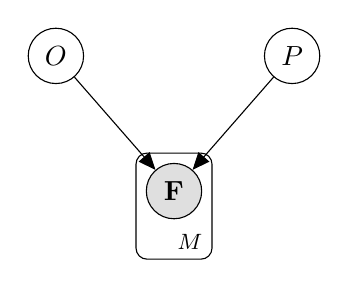
\begin{tikzpicture}
            % Define nodes
            \node[obs]                            (F) {$\set{F}$};
            \node[latent, above=of F, xshift=-1.5cm] (O) {$O$};
            \node[latent, above=of F, xshift=1.5cm]  (P) {$P$};

            % Connect the nodes
            \edge {P,O} {F};

            % Plates
            \plate {} {(F)} {$M$}
          \end{tikzpicture}
          \caption{Simple object recognition graph.}
          \label{fig:objectRecognitionSubgraph}
        \end{figure}

        The likelihood of a feature, $\prob{f|o,p}$ is a distribution derived from feature matching errors. Each feature in the model has an associated type $j$ and a value or descriptor with which to compute a similarity or matching error $\cursive{E}^j(\cdot,\cdot)$ with respect to another feature of the same type.

        The features of this model are selected as the set of all unique features observed in an ideal setting for all objects and poses in the model. 

        % OLD
            % Before training this model, we first must construct the structure of this model. We selected a set of objects and chose a number of poses we wanted the model to learn. We gathered a set of features for each object-pose pair in an ideal setting to create an initial dataset.
            % % I would introduce a term here. Like a database for example. So that we can refer to it later.

            % \begin{equation}
            %     \cursive{D} = \left\{ \left(o_k,p_k,\set{F}_k\right)^{k=K}_{k=1} \right\}
            % \end{equation}

            % % I think that this indexing with k is confusing. because now it seems that there is k objects.. I know what you want to say. But I think I would even remove this. Also, structure of a model sounds like we want to infer the structure of the graph...

            % The model was constructed as set of all unique objects, poses, and features observed in $\cursive{D}$. % I dont really understand this sentence. What is the model exactly?

        Given an observation, $\set{F}_{\text{obs}}$, the best matching error with respect to a feature in the model $f^j \in \set{F}$ is given by \eqref{eq:bestMatch}.
     	% I put new commands in for referencing equations, figures and so on. Please use those.    
            % matching, descriptors - these are very SIFT-like terms. I don't think one can understand what we mean by matching now. That's why I would also move away from being so generic and just concentrate on our features. At the end we can mention that it is also extendable to other feature types.
        \begin{equation}
            \label{eq:bestMatch}
            \cursive{E}(f^j) = \min_{f^j_{\text{obs}} \in \set{F}_{\text{obs}}}\cursive{E}^j(f^j,f^j_{\text{obs}})
        \end{equation}
        
        Training data consists of $R$ sets of feature observations for each object-pose pair. The feature likelihood distribution is learned from the distribution of best matching errors across all training observations for a specific object-pose.
        % We compute a set of best matching errors for each feature in the model across all training samples and learn the distribution of these errors.
        \begin{equation}
            \prob{f|o,p} \sim \{\cursive{E}_1(f), ...,  \cursive{E}_R(f)\}
        \end{equation}
        Note that this procedure works for any type of feature given an error function. This model can also combine multiple feature types into a single object recognition model. For our model, we used only SIFT features and learned a normal distribution for the feature likelihood.   
        \begin{equation}
            \prob{f|o,p} \sim \cursive{N}(\mu,\sigma)
        \end{equation}
        % OLD
            % \begin{equation}
            %     \prob{f_m|o_n,p_i} \sim \cursive{N}(\mu_{m}^{n,i},\sigma_{m}^{n,i})
            % \end{equation}
            % I would remove the m index here. It doesnt help much and it's not easily readable
        % \subsubsection{Object-Pose Inference}
        
        The posterior for predicting object-pose is given by the posterior in \eqref{eq:firstPosterior}.
        \begin{equation}
            \label{eq:firstPosterior}
            \prob{o,p|\set{F}} = \frac{\prob{o,p} \cdot \prob{\set{F}|o,p}}{\prob{\set{F}}}
        \end{equation}
        Based on the assumption that features are conditionally independent given object and pose, the joint feature likelihood can be computed as a product shown in \eqref{eq:setFeatureLikelihood}.
        \begin{equation}
            \label{eq:setFeatureLikelihood}
            \prob{\set{F}|o,p} = \prod_{m=1}^{M} \prob{f_m|o,p}
        \end{equation}
        Assuming a uniform prior on objects and poses, the posterior can then be computed as shown in \eqref{eq:firstPosteriorComputation}.
        \begin{equation}
            \label{eq:firstPosteriorComputation}
            \prob{o,p|\set{F}} = \frac{\prob{\set{F}|o,p}}{\sum_{n,i} \prob{\set{F}|o_n,p_i}}
        \end{equation}
    \subsection{Action Selection Model}
        For action selection, we extend the object-recognition subgraph into a time-series graph. Actions are modeled as $I$ pairwise relative pose transformations including the \italic{stay} action to determine when the algorithm has converged. The next pose, $P_{t+1}$ is dependent only on the previous pose, $P_t$ and the previous action $A_t$. This results in a graphical model shown in \figref{fig:fullGraph}.
        \begin{figure}[h]
          \centering
          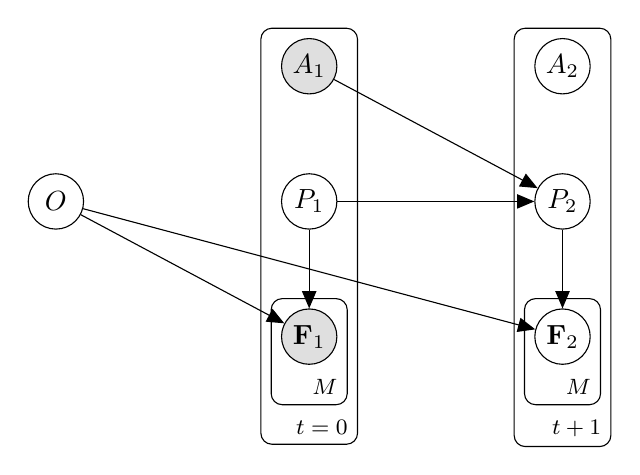
\begin{tikzpicture}
            % Define nodes
            \node[obs] (F) {$\set{F}_1$};
            \node[latent, above=of F]  (P) {$P_1$};
            \node[latent, left=of P, xshift=-1.5cm] (O) {$O$};
            \node[obs, above=of P]  (A) {$A_1$};

            \node[latent, right=of F, xshift=1.5cm] (F2) {$\set{F}_2$};
            \node[latent, above=of F2]  (P2) {$P_2$};
            \node[latent, above=of P2]  (A2) {$A_2$};


            % Connect the nodes
            \edge {P,O} {F};
            \edge {P2,O} {F2};
            \edge {P,A} {P2};

            % Plates
            \plate {pf} {(F)} {$M$}
            \plate {pf2} {(F2)} {$M$}

            \plate {} {(F)(P)(A)(pf)} {$t=0$}
            \plate {} {(F2)(P2)(A2)(pf2)} {$t+1$}
          \end{tikzpicture}
          \caption{graph model}
          \label{fig:fullGraph}
        \end{figure}
        % \begin{figure}[h]
        %   \centering
        %   \begin{tikzpicture}
        %     % Define nodes
        %     \node[obs] (F) {$\set{F}_1$};
        %     \node[latent, above=of F]  (P) {$P_1$};
        %     \node[latent, left=of P, xshift=-1.5cm] (O) {$O$};
        %     \node[obs, above=of P]  (A) {$A_1$};

        %     \node[obs, right=of F, xshift=1.5cm] (F2) {$\set{F}_2$};
        %     \node[latent, above=of F2]  (P2) {$P_2$};
        %     \node[obs, above=of P2]  (A2) {$A_2$};

        %     \node[latent, right=of F2, xshift=1.5cm] (F3) {$\set{F}_3$};
        %     \node[latent, above=of F3]  (P3) {$P_3$};
        %     \node[latent, above=of P3]  (A3) {$A_3$};


        %     % Connect the nodes
        %     \edge {P,O} {F};
        %     \edge {P2,O} {F2};
        %     \edge {P3,O} {F3};
        %     \edge {P,A} {P2};
        %     \edge {P2,A2} {P3};

        %     % Plates

        %     \plate {pf} {(F)} {$M$}
        %     \plate {pf2} {(F2)} {$M$}
        %     \plate {pf3} {(F3)} {$M$}

        %     \plate {} {(F)(P)(A)(pf)} {$t=1$}
        %     \plate {} {(F2)(A2)(pf2)} {$t=2$}
        %     \plate {} {(F3)(A3)(pf3)} {$t=3$}

        %     \draw [dotted, thick] (7.5,1.5) -- (7.85,1.5);
        %   \end{tikzpicture}
        %   \caption{Generalized Model}
        %   \label{fig:fullGraph}
        % \end{figure}

        % \subsubsection{First Action}
        % After initially observing data $\set{F}_1$, we compute the posterior for all object-poses. We consider what is the optimal action $a \in A_1$ which would lead to a new pose $P_2$ and reveal new features $\set{F}_2$. This joint distribution is factorized by equation \ref{eq:firstActionFactorized}, depicted in figure \ref{fig:firstActionGraph}.

        % \begin{multline}
        %     \label{eq:firstActionFactorized}
        %     \prob{O,P_1,P_2,\set{F}_1, \set{F}_2, A_1} = \\ \prob{O}\prob{P_1}\prob{\set{F}_1|O,P}\prob{P_2|P_1|A_1}\prob{\set{F}_2|O,P_2}
        % \end{multline}

        %we can show how posterior looks for one action but after that let's stay with the generic formulation. Also with the graph - it should definitely be for n. That way it is more professional

        % The posterior for the after the first action is computed as a simple update of the first posterior shown in equation \ref{eq:firstActionPosterior}.

        % \begin{multline}
        %   \label{eq:firstActionPosterior}
        %   \prob{o|\set{F}_1,\set{F}_2,a} = \\ \frac{\sum_{P_1,P_2} \prob{o,P_1|\set{F}_1} \; \prob{\set{F}_2|P_2,o} \; \prob{P_2|P_1,a}}{\sum_{P_1,P_2,O} \prob{O,P_1|\set{F}_1} \; \prob{\set{F}_2|P_2,O} \; \prob{P_2|P_1,a}}
        % \end{multline}

        % To determine the optimal action we compute the minimum expected entropy of object prediction for the distribution in equation \ref{eq:firstActionPosterior} given by equation \ref{eq:firstActionOptimal}.
        %TODO: we need more explanation on this. Why expected entropy? why does it work?

        % \begin{equation}
        %   \label{eq:firstActionOptimal}
        %   a^* = \argmin_{A_1} \expectedValue{\entropy{O|\set{F}_1,\set{F}_2,A_1}}{\set{F}_2 \sim \prob{\set{F_2}|\set{F}_1,A_1}}
        % \end{equation}

        % \subsubsection{Generalized Optimal Action}
        
        The posterior at time $t+1$ given the entire history of observations and actions is simply a Bayesian update of the posterior at time $t$ given in \eqref{eq:fullPosterior}.
        \begin{multline}
            \label{eq:fullPosterior}
            \prob{o,P_{t+1}|\set{F}_{1:t+1},A_{1:t}} = \\ \frac{ \sum_{P_t} \prob{o,P_t|\set{F}_{1:t},A_{1:t-1}} \prob{\set{F}_{t+1}|o,P_{t+1}} \prob{P_{t+1}|P_t,A_t}}{\sum_{P_t,P_{t+1},O} \prob{O,P_t|\set{F}_{1:t},A_{1:t-1}} \prob{\set{F}_{t+1}|O,P_{t+1}} \prob{P_{t+1}|P_t,A_t}}
        \end{multline}
        For our experiment, we consider actions to be perfect, i.e. $\prob{P_{t+1}|P_t,A_t} \in \{ 0 , 1 \}$. Thus, given an action and a pose, the next pose can be computed deterministically. This simplifies our Bayesian update to \eqref{eq:fullPosteriorSimplified}.
        \begin{multline}
            \label{eq:fullPosteriorSimplified}
            \prob{o,P_{t+1}|\set{F}_{1:t+1},A_{1:t}} = \\ \frac{\prob{o,P_t|\set{F}_{1:t},A_{1:t-1}} \prob{\set{F}_{t+1}|o,P_{t+1}} }{\sum_{P_t,O} \prob{O,P_t|\set{F}_{1:t},A_{1:t-1}} \prob{\set{F}_{t+1}|O,P_{t+1}} }
        \end{multline}
        
        We defined the optimal action as moving an object into the least ambiguous pose resulting in a minimum entropy across predicted object probabilities. The posterior object probability $\prob{o|\set{F}_{1:t+1},A_{1:t}}$ is a distribution because we have not observed $\set{F}_{t+1}$. Thus, we minimize the \italic{expected} entropy of this posterior for all potential actions given by \eqref{eq:optimalAction}.
        \begin{equation}
            \label{eq:optimalAction}
            a^* = \argmin_{A_t} \expectedValue{ \entropy{O|\set{F}_{1:t+1},A_{1:t}} }{\set{F}_{t+1} \sim \prob{\set{F_{t+1}}|\set{F}_{1:t},A_{1:t}}}
        \end{equation}
        That can be efficiently computed with a particle filter approximate sampling method.

        % OLD
            % \subsubsection{Implementation}

            % This algorithm follows a simple posterior update rule
            % \begin{align}
            %     \text{posterior}_t &= \frac{\text{posterior}_{t-1}*\text{likelihood}_t}{\text{evidence}_t}\\
            %     &= \frac{\text{posterior}_{t-1}*\text{likelihood}_t}{\sum \text{posterior}_{t-1}*\text{likelihood}_t}
            % \end{align}

            % \begin{table}[h]
            %   \begin{tabular}{c|c|c|c} % number of columns and vertical lines
            %     \hline % top horizontal line
            %     Time & Posterior & Evidence & Likelihood\\
            %     [0.5ex] % [0.5ex] adds vertical space
            %     \hline\hline % inserts double-line
            %     0 & $\prob{o,p}$ & & \\[0.5ex] 
            %     1 & $\prob{o,p|\set{F}_1}$ & $\prob{\set{F}_1}$ & $\prob{\set{F}_1|o,p}$ \\[0.5ex] 
            %     2 & $\prob{o,p|\set{F}_1,\set{F}_2,A_1}$ & $\prob{\set{F}_2|\set{F}_1,A_1}$ & $\prob{\set{F}_2|o,p}$ \\
            %     ...&...&...&...\\[0.5ex] 
            %     t & $\prob{o,p|\set{F}_{1:t},A_{1:t-1}}$ & $\prob{\set{F}_t|\set{F}_{1:t-1},A_{1:t-1}}$ & $\prob{\set{F}_t|o,p}$
            %   \end{tabular}
            %   % \label{tab:updateRule}
            %   % \caption{Update cache}
            % \end{table}

            % Our implementation uses a particle filter for computing the optimal action.
            % this is not a particle filter stricte but we use MCMC method to approximate distributions. Also, we shouldn't put implementation in.

        % include derivations in the appendix

\section{Experimental Results}

    We evaluated the proposed approach on a dataset consisting of 4 books, two of which looking the same from the back. Each book was trained in 4 discrete poses being: cover up with visible spine, cover up with no visible spine, cover down with visible spine and cover down with no visible spine. For each object-pose pair we extracted approximately 50 SIFT features which are later used for feature matching. We took 100 training images of each object-pose pair to learn the distribution ADD EQ REF. For the ambiguous case (the book looks the same from the cover down pose) we use the same training images as the books look the same from that side.

    Our experimental setup consists of a Microsoft Kinect sensor which we use as a RGB camera and one of the objects from the database. All the actions are executed by a human and we assume that there is no noise in the action execution. 

    \subsection{Object Recognition}
        %*cross validation error,

    \subsection{Action Selection}
        The experiment is constructed as follows. We expose an object to the Kinect sensor and obtain the recognition result. In the next step we employ the action selection algorithm to choose the best action and we execute it. In order to measure if the action improved the previous recognition we compute the posterior probability of the object. TABLE REF presents the posterior probabilities of the object as well as the best action that was chosen by the algorithm. We execute actions until the algorithm converges which means that the action selection algorithm returns says that all the actions are equally informative.

        We ran the above described experiment in various conditions, i.e. different books and different starting poses(ambiguous and non-ambiguous). The results are described in TABLE REF.
        
        DISCUSSION


        %*explain our setup
        % we have a kinect, 4 object, 4 poses each, 50 sift features per object-pose pair
        % 100 training images per object-pose pair
        % we move the object with our hands for now
        %  

        %*assumptions
        % perfect actions (no noise)
        % discrete poses 
        % we see one object at a time
        % we see a known object

        %*explain experiment
        % we show the object to the kinect and recognize it based on our recognition module
        % results for all objects and poses are in the table
        % we figure out the best action (in the table)
        % we check recognition after the action has been taken (in the table)


%        \begin{itemize}
%        \item explain our dataset
%        \item show pictures of objects
%        \item show cross validation results for our training
%        \item explain the setup
%        \item show real data results for object recognition (table)
%        \item discuss the results, emphasize that the action selection works
%        \end{itemize}

        \section{Conclusions}
        \begin{itemize}
        \item discuss the results
        \item what failed what succeeded
        \item talk about possible extensions: continuous pose, more feature types, on the robot
        \end{itemize}

\section*{Acknowledgments}

    \cite{McGeer01041990}


%% Use plainnat to work nicely with natbib. 

\bibliographystyle{plainnat}
\bibliography{references}

\end{document}


